\documentclass[12pt]{exam}
%\documentclass[12pt]{article}
\usepackage[letterpaper, margin=0.75in]{geometry}
\usepackage{graphicx}
\usepackage{enumitem}
\usepackage{booktabs}
\usepackage{amsmath}
\usepackage{tabularx}
\usepackage{color}

\begin{document}
\footer{}{Page \thepage\ of \numpages}{}

\begin{flushright}
\makebox[0.5\textwidth]{\large Name:\enspace\hrulefill}
\vspace{0.2in}

\makebox[0.5\textwidth]{\large Date:\enspace\hrulefill}
\end{flushright}

\begin{center}

\includegraphics[width=10cm]{../images/logo.png}
\end{center}

\begin{center}
\noindent{\LARGE Conceptual Physics \\ Class 10 Questions \\ April 13th, 2018 \\}
\end{center}

\noindent\textbf{\Large Some Useful Facts:}
\begin{enumerate}
\item The speed of light is $3\times 10^8 m/s$
\item The distance between the Earth and the Sun is about 8 light-minutes
\item The distance between the Earth and the Moon is about 1.5 light-seconds
\end{enumerate}

\clearpage

\begin{questions}
\question Two \textit{positive charges} are held close together. The following 4 panes will ask you do draw different things, but they are all for the same pair of positive charges.
\begin{center}
	\input{../images/4panePositiveCharges.pdf_tex}
\end{center}

\clearpage
\question A positive (blue) and a negative (red) charge are held close together. The following 4 panes will ask you do draw different things, but they are all for the same pair of charges.
\begin{center}
	\input{../images/4pane2Charges.pdf_tex}
\end{center}

\clearpage
\question Why do actions at a distance have a time delay?
\vspace{1in}

\question Are forces transmitted instantaneously? Why or why not?
\vspace{1in}

\question List 3 examples of fields.
	\begin{parts}
		\part 
			\vspace{0.1in}
		\part 
			\vspace{0.1in}
		\part 
	\end{parts}

\vspace{0.5in}

\question We discussed electric and gravitational fields, since fields are associated with forces. Friction is a (contact) force. Is there such a thing as a ``friction field"?
\vspace{1in}

\question A (still) proton and an electron are separated by a distance of 9~m. The proton is then jiggled up and down. How long will it take for the electron to experience a change in the electric force as a result of the proton's jiggling?
\vspace{1in}

\clearpage
\question You are standing on the Earth, and notice the Moon orbiting in the sky. If the Earth were to suddenly vanish beneath you, what would you notice about the moon's motion?
\vspace{1in}

\question When finding the strength of a gravitational field, does the size of the test mass matter? Why or why not?
\vspace{1in}

\question When finding the strength of an electric field, does the charge on the test charge matter? Why or why not?
\vspace{1in}

\question A 2~kg rock is held on the surface of the moon, whose gravitational field is much weaker than Earth's. If the gravitational field at the point of the rock is $1.6~m/s^2$ down, what force does the rock experience?
\vspace{1in}

\question In order to find the strength of the gravitational field on Mars, a 10~kg test mass is held 1~m off the ground, and experiences a weight of 37~N. What is the strength of the gravitational field on the surface of Mars?
\vspace{1in}

\clearpage
\question Use the diagram below to answer the following:
\begin{parts}
	\part A ``sea of arrows" representing the gravitational field around the Earth.
	
		\vspace{1.5in}
			\begin{center}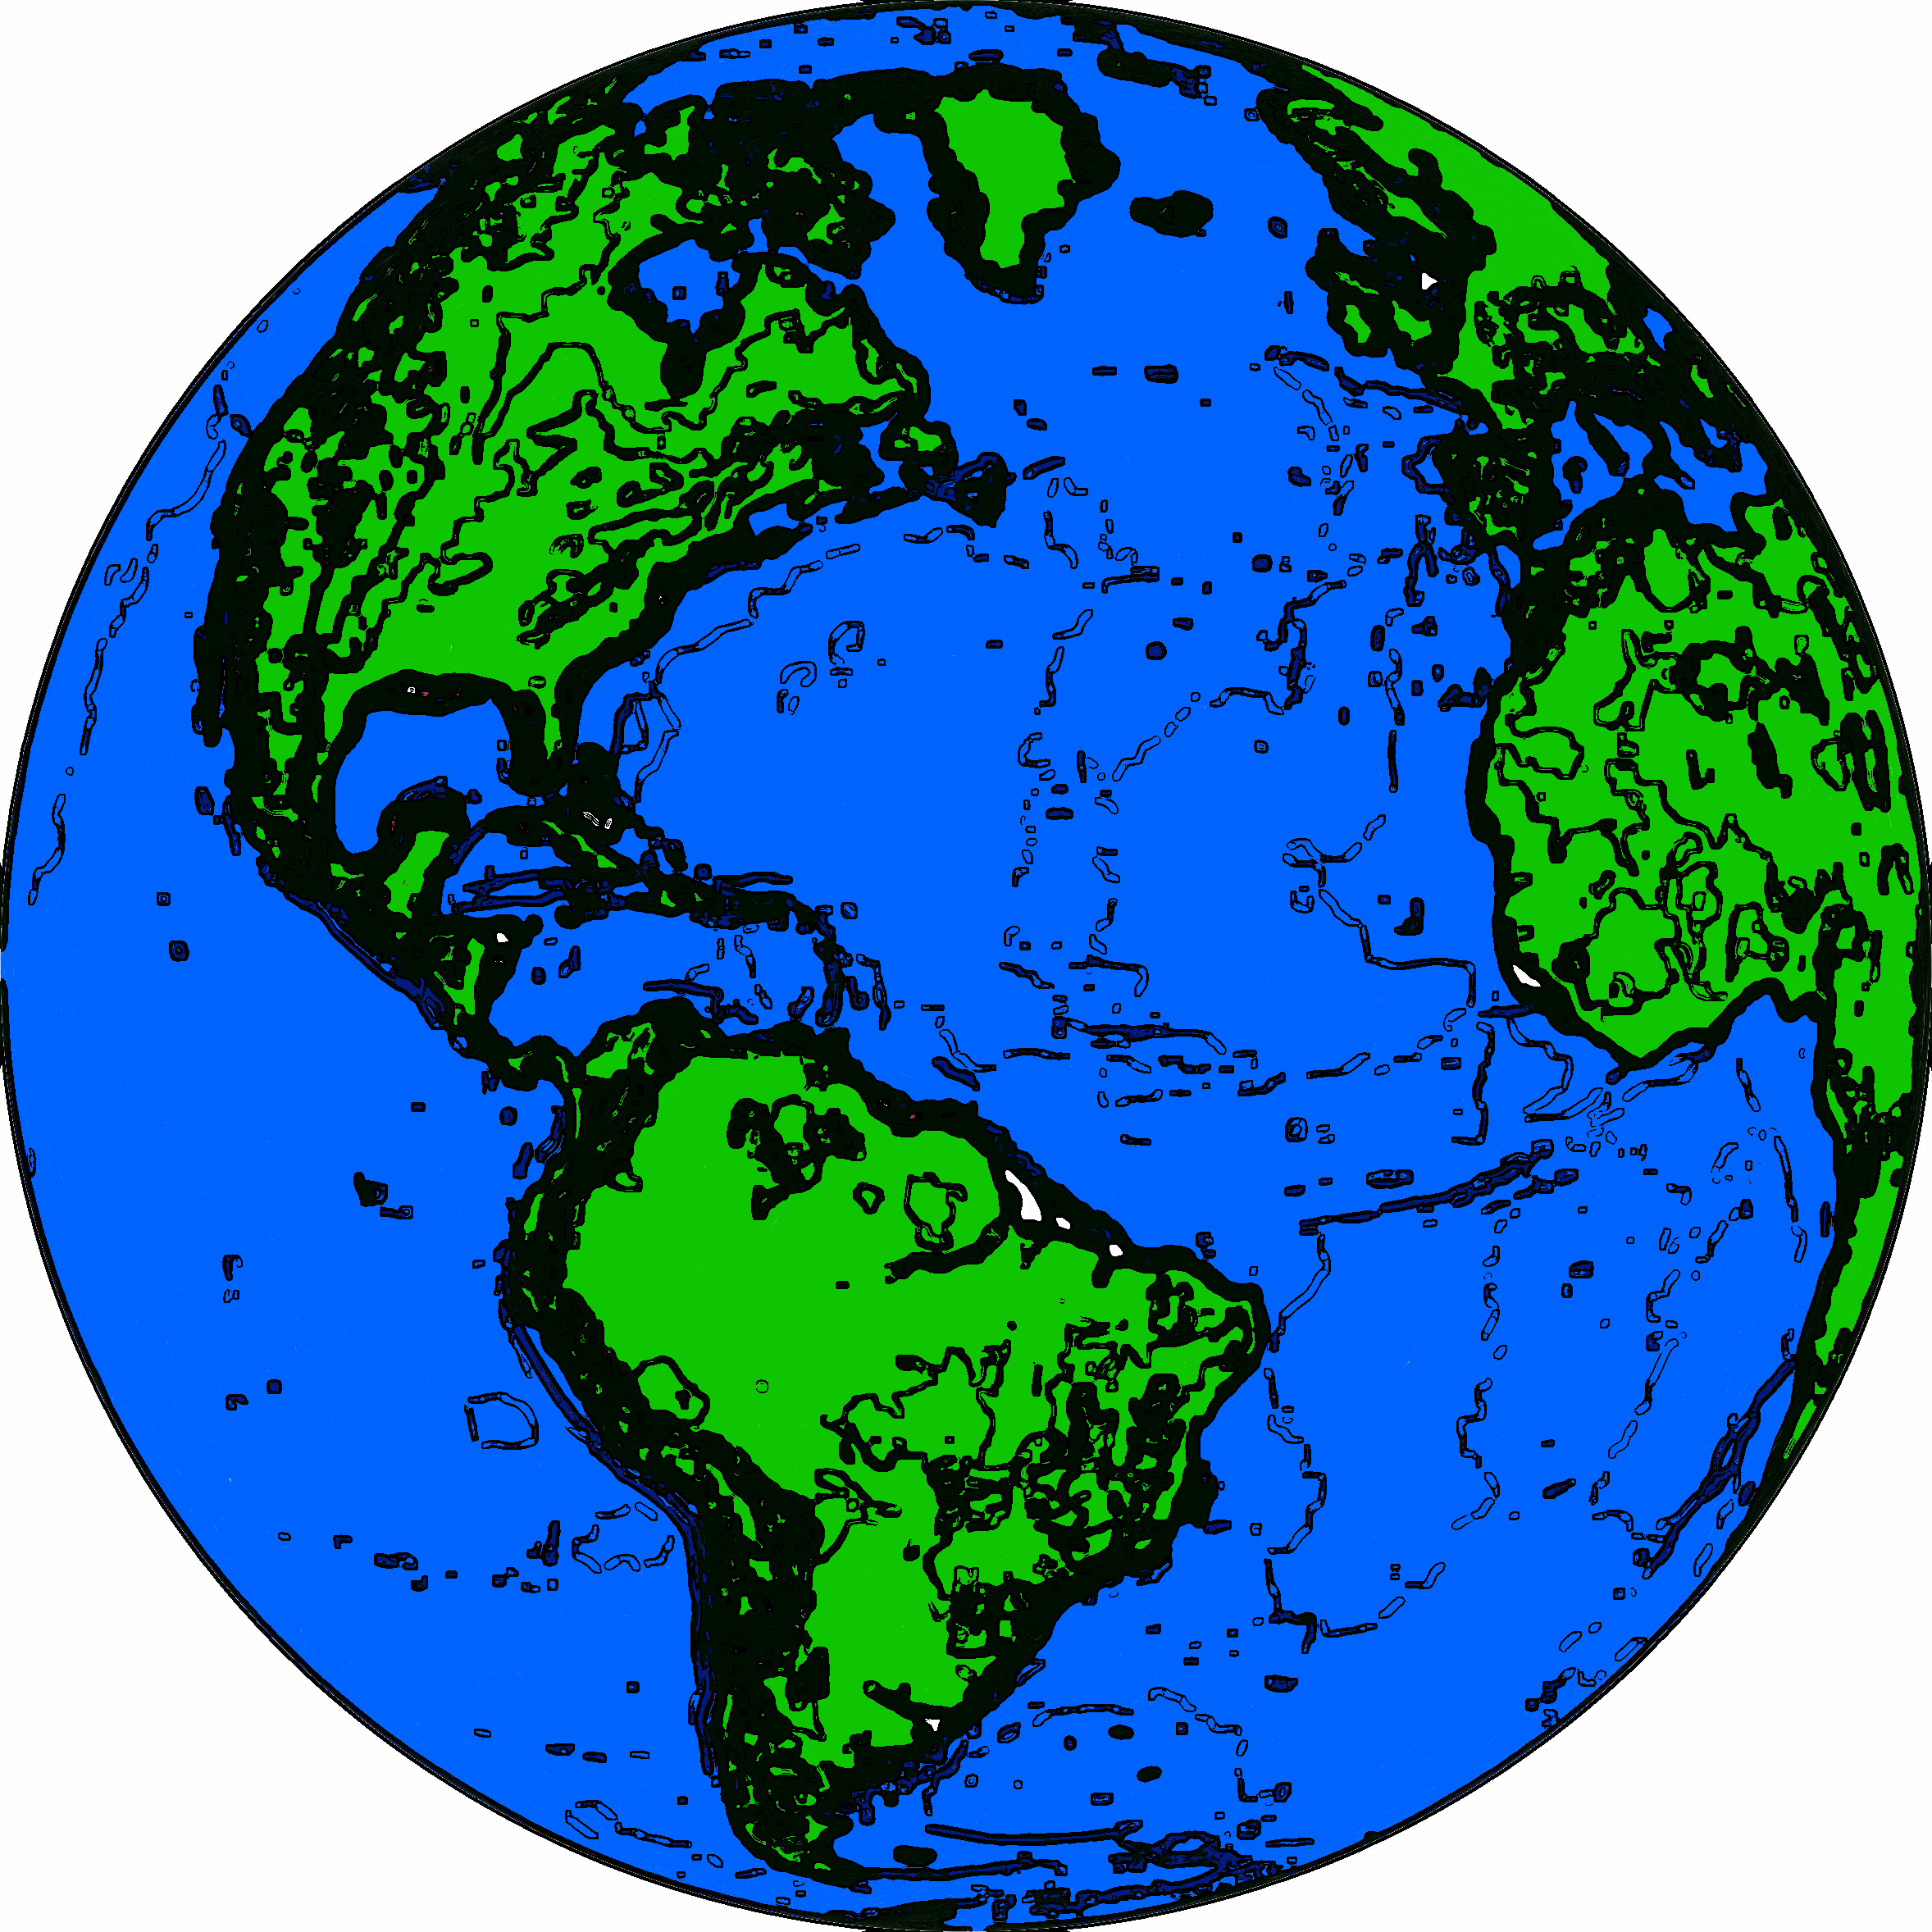
\includegraphics[width=0.5in]{../images/earth.png}\end{center}
		\vspace{1.5in}
		
	\part Field lines representing the gravitational field around the Earth.
	
		\vspace{1.5in}
			\begin{center}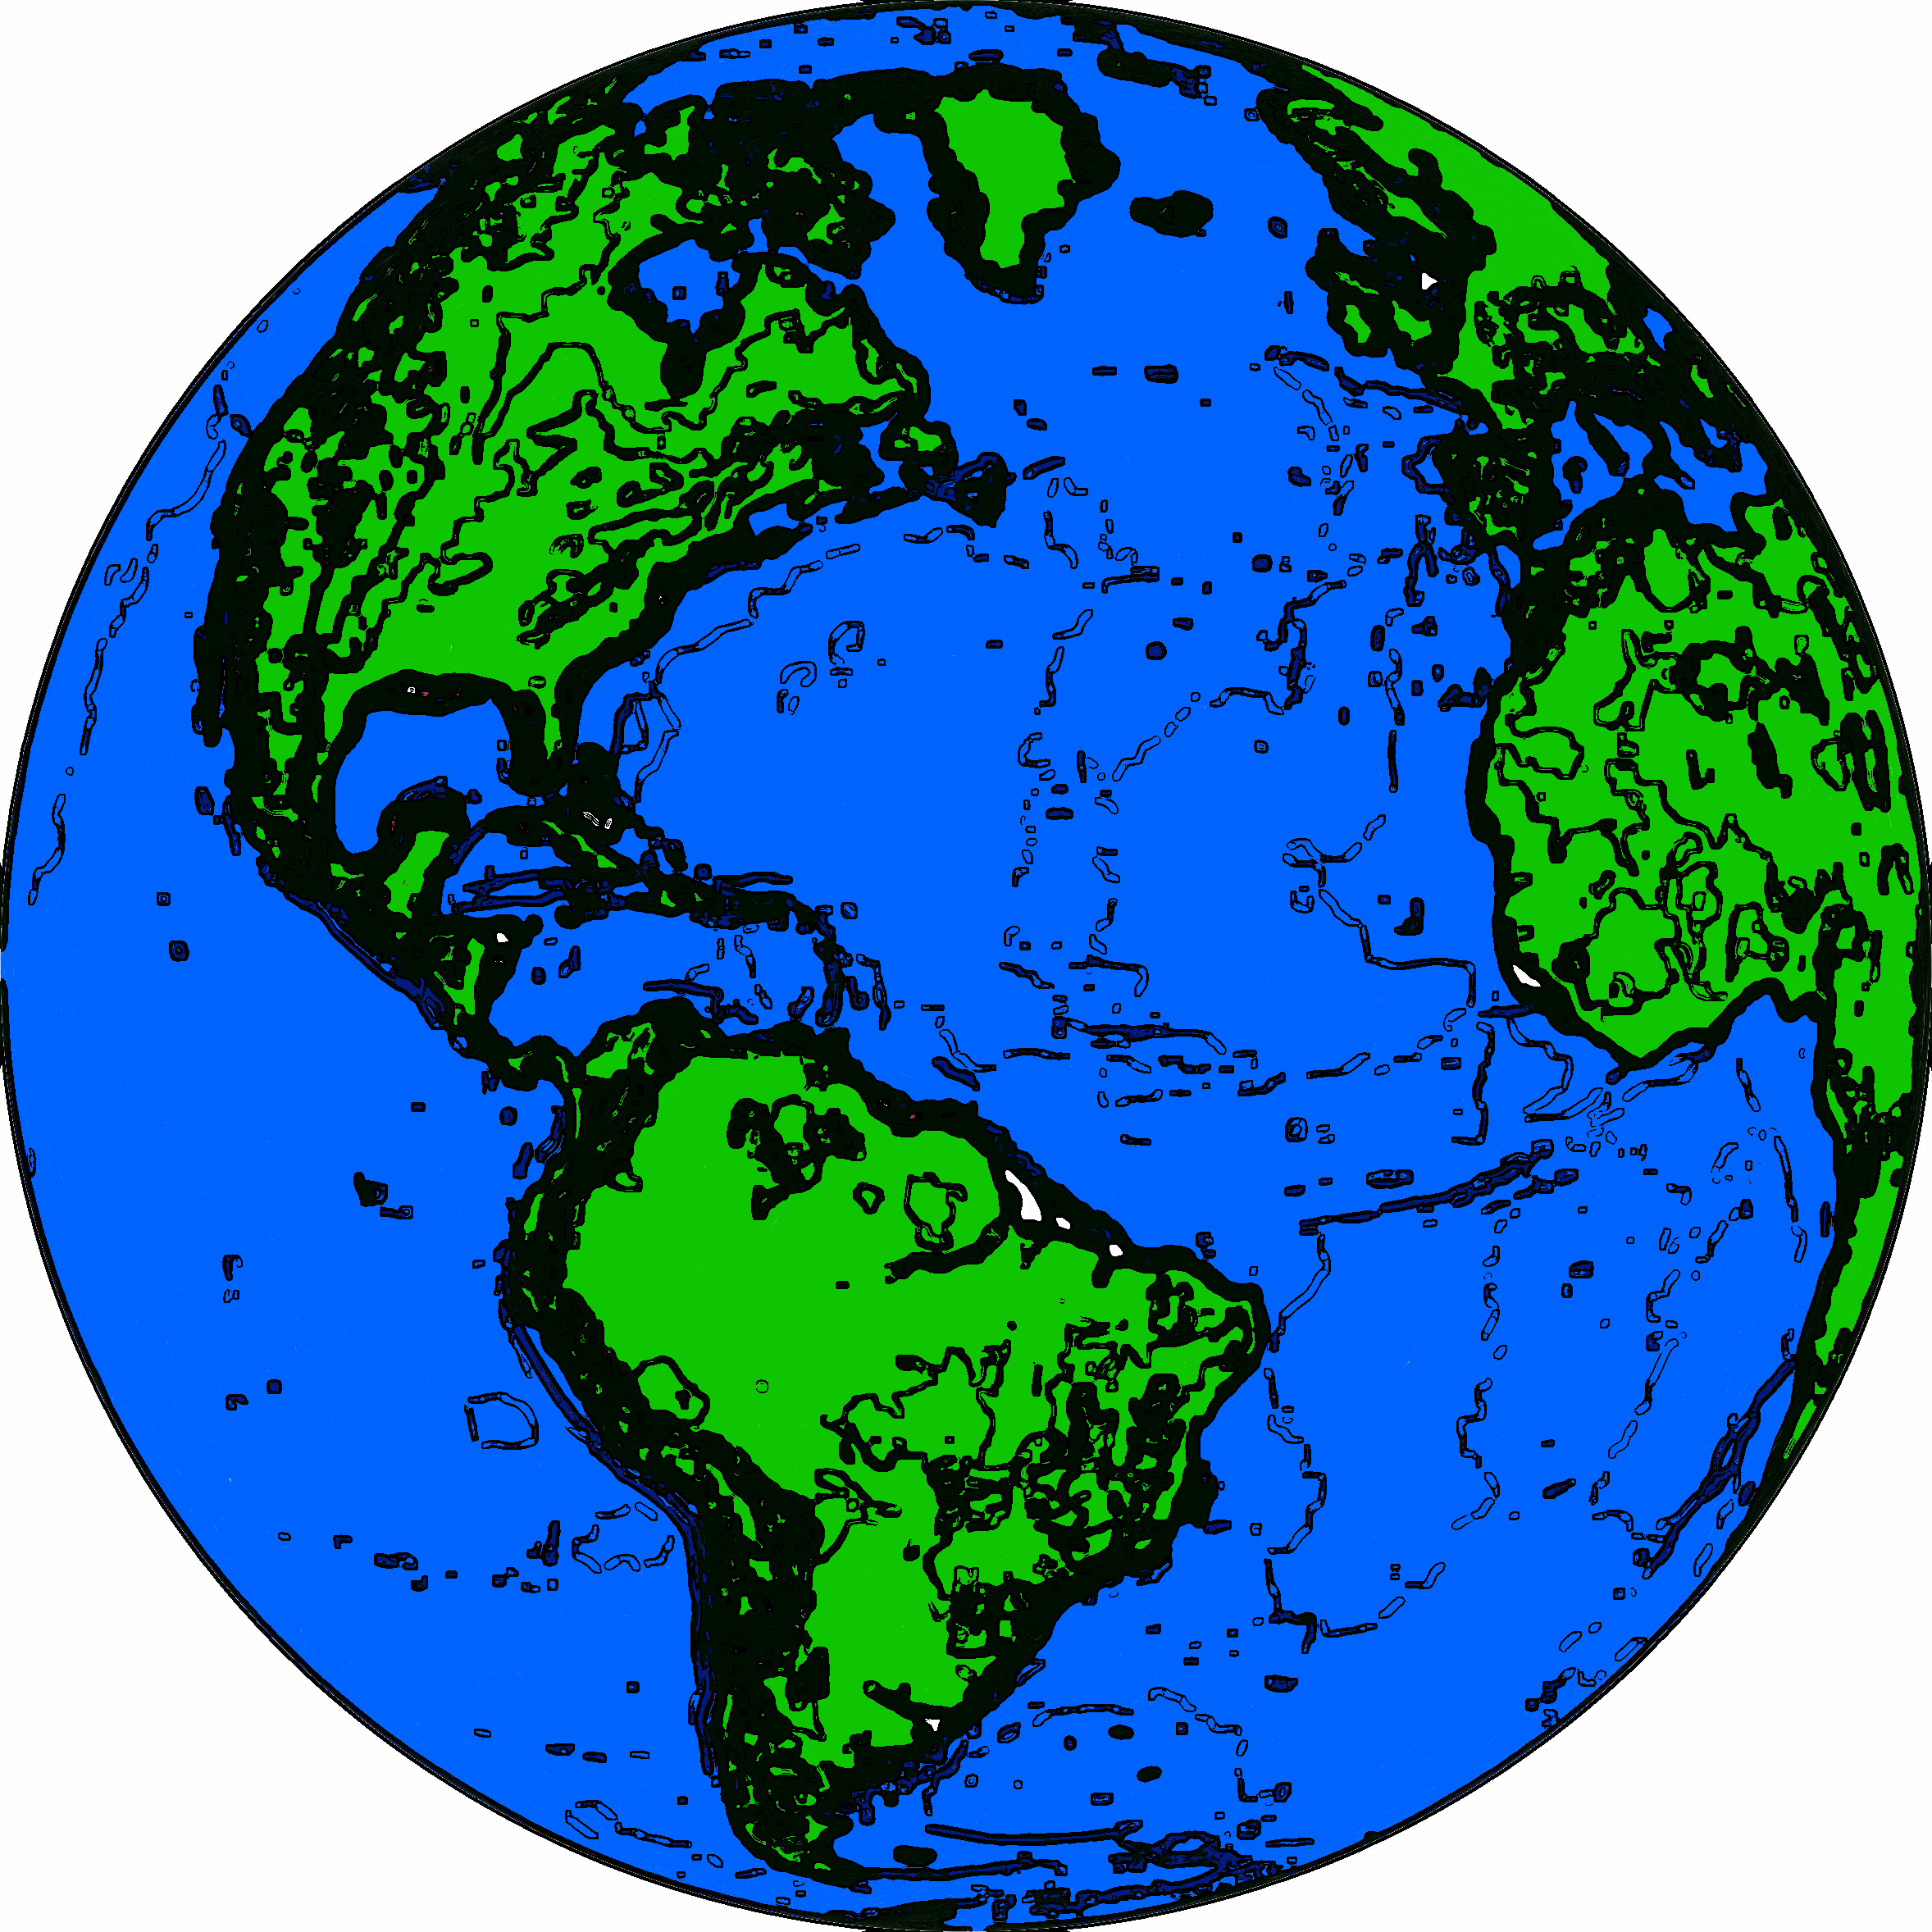
\includegraphics[width=0.5in]{../images/earth.png}\end{center}
		\vspace{1.5in}
\end{parts}

\clearpage
\question What is the difference between a \textit{source} and a \textit{sink} for field lines?
\vspace{1in}

\question Draw the electric field lines around:
\begin{parts}
	\part A proton (positively charge particle). Is a proton a source or a sink?
	
		\vspace{1.5in}
			\begin{center}
\includegraphics[width=0.1in]{../images/proton.png}\end{center}
		\vspace{1.5in}
	
	\part An electron (negatively charged particle). Is an electron a source or a sink?
	
		\vspace{1.5in}
			\begin{center}
\includegraphics[width=0.1in]{../images/electron.png}\end{center}
		\vspace{1.5in}
\end{parts}

\clearpage
\question An object has some mass and a positive charge, as shown bellow.
\begin{parts}
	\part Draw an arrow representing the direction of the \textbf{gravitational field} at point \textit{A}.
	\part Draw an arrow representing the direction of the \textbf{electrical field} at point \textit{A}.
	\part A test mass with a \textit{negative} charge is placed at point \textit{B}. Draw an arrow representing the \textbf{gravitational force} experienced by this test mass, as well as another arrow representing the \textbf{electrical force}.
\end{parts}

\vspace{2in}
\begin{center}
\input{../images/testChargeMass.pdf_tex}
\end{center}

\clearpage
\question Two metal plates are floating in space, separated by some distance.
\begin{parts}
	\part If the top plate has a positive charge, and the bottom plate has a negative charge, draw the field lines representing the \textit{electric field} surrounding the two plates.
	\vspace{1in}
	\begin{center}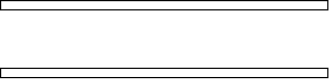
\includegraphics[width=2in]{../images/2plates.png}\end{center}
	\vspace{1in}
	
	\part If both plates have a positive charge, draw field lines representing the \textit{electric field}. What is the strength of the electric field at a point exactly midway between the two plates?
	\vspace{1in}
	\begin{center}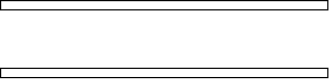
\includegraphics[width=2in]{../images/2plates.png}\end{center}
	\vspace{1in}
	
	\part Draw field lines representing the \textit{gravitational field.} What is the strength of the gravitational field at a point exactly midway between the two plates?
	\vspace{1in}
	\begin{center}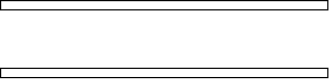
\includegraphics[width=2in]{../images/2plates.png}\end{center}
	\vspace{1in}
\end{parts}

	
\end{questions}

\end{document}
